% Number 440
% UFPM Tension
% pulling mass up with string - easy
% MIT

% Watermark
\AddToShipoutPicture*{\BackgroundPic}

\addtocounter {ProbNum} {1}

%\begin{floatingfigure}[r]{.35\textwidth}
%\includegraphics[scale=.5]{/Users/jgates/desktop/latex/pics/staticeq1.png}
%\end{floatingfigure}
 
{\bf \Large{\arabic{ProbNum}}} A 2.45 kg mass is suspended from a string which is pulled upward. The mass accelerates upwards with an acceleration of ${2.3~\tfrac{m}{s^2}}$. 
\bigskip
What is the tension in the string?

%\begin{center}
%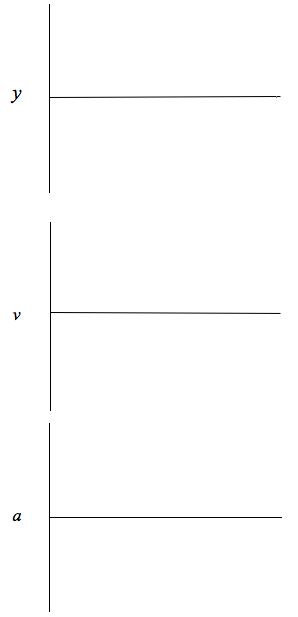
\includegraphics[scale=.85]{/Users/jgates/desktop/latex/pics/blankyvagraphstack.png}
%\end{center}


\vfill
\newpage